%% Ecological Informatics — IMRaD manuscript (Overleaf-ready)

\documentclass[preprint,12pt,3p,times]{elsarticle}

\usepackage{amssymb}
\usepackage{amsmath}
\usepackage{graphicx}
\usepackage{booktabs}
\usepackage{multirow}
\usepackage{url}
\usepackage{hyperref}
\usepackage{lineno}
\usepackage{xcolor}

\journal{Ecological Informatics}

\begin{document}

\begin{frontmatter}

\title{A fine-grained re-identification approach for Asian elephants with morphological feature-region supervision}

\author[inst1]{First Author}
\author[inst1]{Second Author\corref{cor1}}
\ead{corresponding.author@institution.edu}

\author[inst2]{Third Author}

\address[inst1]{Department of [PLACEHOLDER], [University], [City], [Country]}
\address[inst2]{[Facility / Research Centre], [City], [Country]}

\cortext[cor1]{Corresponding author.}

\begin{abstract}
We present a \textbf{fine-grained re-identification approach} for Asian elephants (\textit{Elephas maximus}) that combines EfficientNet-V2-S classification with \textbf{morphological feature-region supervision} and track-level identity stabilisation. Through three successive \textbf{training configurations}---two whole-body-only baselines followed by a proposed body-plus-feature regime---we show that high top-1 accuracy on held-out reference-library crops (99.85\% under the refined body-only configuration) does not guarantee field performance: both body-only models generalised poorly to in-situ photographs and YOLO detector crops, whereas the body-plus-feature configuration markedly improved field re-identification. Generalisation therefore depends on morphological feature-region supervision rather than reference-catalogue metrics alone. At inference, the approach uses a detect--classify--stabilise pipeline (YOLO, intermittent classification, identity caching and lock-after-confidence, optional candidate filtering). The primary evaluation compares reference-library, in-situ, and YOLO-crop accuracy across training configurations.
\end{abstract}

\begin{keyword}
Asian elephant \sep individual re-identification \sep fine-grained classification \sep feature-region supervision \sep morphological feature annotation \sep deep learning \sep domain generalisation \sep transfer learning \sep ecological informatics
\end{keyword}

\end{frontmatter}

%% Highlights — fine-grained re-ID approach (≤85 chars per bullet)

\section*{Highlights}
\begin{itemize}
  \item Fine-grained re-identification approach for Asian elephants
  \item Morphological feature-region supervision with body+feature training
  \item Body-only configs: 99.85\% on reference library but poor field re-ID
  \item Proposed body+feature config substantially improves in-situ recognition
  \item Three-configuration ablation separates library metrics from field gain
\end{itemize}


\section{Introduction}
\label{sec:intro}

Individual re-identification links sequential observations to known animals, enabling inference on residency, association, and behaviour from passive monitoring data \citep{kuhl2014, schofield2019}. For Asian elephants (\textit{Elephas maximus}), expert identification relies on stable morphological traits---ear folds, tusk shape, depigmentation, and scars---but manual review does not scale with the volume of images and video generated by modern camera-trap networks \citep{plotnik2011, weinstein2018, norouzzadeh2021}.

Computational re-identification typically follows a detect-then-classify paradigm: a detector localises animals, and a fine-grained classifier assigns individual labels to cropped regions \citep{schneider2019, tabak2019}. In ecological deployments, however, three gaps persist. First, training data often comprise well-framed reference portraits, whereas inference crops from detectors are noisier and partially occluded. Second, independent per-frame classification in video produces unstable labels despite stable bounding-box tracks. Third, closed-set classifiers trained on facility-specific catalogues may confuse visually similar individuals unless temporal logic and prior knowledge constrain the label space.

We address these gaps using data from \textit{[facility name, location]}, where 17 elephants are individually catalogued. We propose a \textbf{fine-grained re-identification approach} built on EfficientNet-V2-S classification, \textbf{morphological feature-region supervision}, and a detect--classify--stabilise video pipeline. Our \textbf{primary contributions} are the approach and its training paradigm; morphological feature-region labelling supplies the supervisory signal that enables field generalisation. Specifically, we contribute:
\begin{enumerate}
  \item a \textbf{fine-grained re-identification approach} with body-plus-feature joint training whose field performance substantially exceeds whole-body-only counterparts, despite the refined body-only configuration reaching 99.85\% on reference-library validation;
  \item a \textbf{morphological feature-region labelling scheme} (Pascal VOC body plus part-level boxes) and a three-configuration training comparison documenting when catalogue metrics mislead deployment evaluation; and
  \item a supporting detect--classify--stabilise inference stack (YOLO, track-level identity caching, lock-after-confidence, optional candidate filtering) for video re-identification.
\end{enumerate}

The remainder of the paper follows the IMRaD structure. Optional deployment on a cellular camera-trap network with \emph{asynchronous} video upload and cloud-side batch processing is reported separately (Section~\ref{sec:deployment}) and is not required to assess the core re-identification approach.

\section{Materials and methods}
\label{sec:methods}

\subsection{Study system and image data}

The study was conducted at \textit{[facility name, location]}, where 17 adult Asian elephants are individually known.

\subsection{Fine-grained re-identification approach}

Reference images were organised in class-specific folders with Pascal VOC XML annotations. The classifier is an EfficientNet-V2-S fine-grained model (ImageNet pre-trained, replaced classification head) trained with \textbf{feature-region supervision}: each annotation file supplies one body box and, under the extended protocol, part-level boxes labelled \texttt{\{name\}-\{part\}} (trunk, foreleg, ear margin, depigmentation, tusk region, etc.) localising morphological identity cues (Figure~\ref{fig:annotation}). Under the proposed body-plus-feature configuration, each image expands into one body crop plus all feature crops sharing the individual label; the two body-only configurations used body crops only. Validation always used held-out body crops so model selection reflects detector-level inputs at inference.

After parsing and padding under the body-only protocol, the catalogue comprised 6{,}592 body crops (5{,}273 training / 1{,}319 validation; stratified 80/20 split). Most individuals contributed approximately 600 reference images; one individual contributed fewer (332). Under the body-plus-feature configuration, each annotated image yielded one body crop plus zero or more part crops, increasing the effective number of training patches while validation remained on body crops only. Images included daytime views with varying pose, distance, and partial occlusion.

\textit{[Insert ethics statement: observational study, facility permission, no invasive procedures.]}

\subsection{Re-identification inference pipeline}

\textbf{Stage 1---Detection and tracking.} Ultralytics YOLO with the COCO \textit{elephant} class (class id 20) produced bounding boxes on each frame. A multi-object tracker assigned persistent \texttt{track\_id} values across frames in video sequences.

\textbf{Stage 2---Individual classification.} Detector crops (with padding) were classified by an EfficientNet-V2-S backbone (ImageNet pre-trained) with a replaced classification head (dropout + linear layer), yielding a closed-set label among the 17 trained identities.

\textbf{Track-level identity stabilisation.} To mitigate label flicker, each \texttt{track\_id} maintained a cached identity. After a confident assignment, the label was locked and retained across subsequent frames unless disambiguation was required among overlapping tracks. Classification was executed intermittently rather than on every frame to balance accuracy and computational cost.

\textbf{Candidate filtering.} When only a subset of catalogued individuals was expected in the scene, inference was restricted to that candidate set (\texttt{allowed\_elephants}), reducing effective class cardinality without retraining. This prior reflects keeper knowledge of daily herd composition in the study facility.

\subsection{Iterative training and ablation design}

Individual classification was developed through three \textbf{training configurations} (Tables~\ref{tab:runs} and \ref{tab:generalization}), reflecting progressive refinement of annotations and training crops rather than ad hoc relabelling. A critical finding emerged after the two body-only configurations: models that performed well on held-out \emph{reference-library} crops failed to generalise to \emph{field} images and YOLO detector outputs, exposing a domain gap between curated catalogue views and deployment conditions.

\textbf{Configuration A---body-only baseline.} An initial model was trained exclusively on VOC body-box crops using EfficientNet-V2-S and a two-phase transfer-learning schedule (Table~\ref{tab:training}). This configuration established the closed-set labelling pipeline and achieved acceptable separation on reference-library validation, but field trials showed low top-1 accuracy on in-situ photographs.

\textbf{Configuration B---body-only refined.} A second body-only configuration repeated the same crop protocol after dataset consolidation (17 named identities, expanded reference folders) and hyperparameter tuning. Validation again used held-out reference body crops only, reaching 99.85\% top-1 accuracy---yet field recognition remained poor, indicating that high catalogue validation scores can mask poor generalisation to detector-level and in-situ views.

\textbf{Configuration C---body plus feature regions (proposed).} Motivated by the library--field gap, the proposed configuration incorporated part-level VOC boxes (trunk, legs, ear margins, etc.) into \emph{training}: each annotated image contributed one body crop plus all available feature crops, all mapped to the same individual label. Validation remained on reference body crops for checkpoint selection. This checkpoint was retained for deployment because qualitative and quantitative field evaluation showed a \textbf{substantial increase} in recognition accuracy on in-situ images and YOLO-driven video crops relative to Configurations~A and~B (\textit{[populate Table~\ref{tab:generalization}]}). The preceding body-only checkpoint was archived before overwriting (\texttt{best\_elephant\_model\_body\_only\_backup.pth}).

Within each configuration, optimisation followed the same two-phase schedule (Table~\ref{tab:training}).

\begin{table}[t]
  \centering
  \caption{Training configurations compared in the ablation. Library validation: held-out reference body crops ($N{=}2{,}073$, stratified 80/20 split, seed~42; VOC body crop, top-1). Field / YOLO rows remain to be completed on in-situ and detector-crop test sets.}
  \label{tab:runs}
  \begin{tabular}{@{}llcc@{}}
    \toprule
    Config. & Training crops & Library val top-1 (\%) & Field / YOLO top-1 (\%) \\
    \midrule
    A & Body only (baseline) & --- & Low \\
    B & Body only (refined) & 75.2 & Low \\
    C & Body + feature (proposed) & \textbf{97.4} & \textit{[TBD]} \\
    \bottomrule
  \end{tabular}
\end{table}

\begin{table}[t]
  \centering
  \caption{Generalisation comparison between Configuration~B (\texttt{best\_elephant\_model\_body\_only\_backup.pth}) and Configuration~C (body plus feature, proposed) on a common evaluation protocol ($N{=}2{,}073$ held-out reference body crops; 17 identities; VOC body crop; seed~42). In-situ and YOLO rows: \textit{to be completed}.}
  \label{tab:generalization}
  \begin{tabular}{@{}lrrr@{}}
    \toprule
    Evaluation domain & Config.\ B & Config.\ C & $\Delta$ (C $-$ B) \\
    \midrule
    Reference-library body val & 75.2 & \textbf{97.4} & \textbf{+22.2} \\
    In-situ / field photographs & \textit{[TBD]} & \textit{[TBD]} & \textit{[+TBD]} \\
    YOLO crops (video frames) & \textit{[TBD]} & \textit{[TBD]} & \textit{[+TBD]} \\
    \bottomrule
  \end{tabular}
\end{table}

\begin{table}[t]
  \centering
  \caption{Two-phase transfer-learning schedule (applied within each training configuration).}
  \label{tab:training}
  \begin{tabular}{@{}lll@{}}
    \toprule
    Phase & Setting & Purpose \\
    \midrule
    1 & Frozen backbone, train head (12 epochs) & Learn identity boundaries \\
    2 & Fine-tune full network (30--40 epochs) & Adapt low-level features \\
    \bottomrule
  \end{tabular}
\end{table}

Training used random resized crops (input size $384\times384$), horizontal flip, colour jitter, label smoothing (0.08--0.10), AdamW optimiser, and cosine learning-rate decay. The best checkpoint within each configuration was selected by maximum validation top-1 accuracy on body crops.

\subsection{Optional deployment context: asynchronous camera-trap video review}
\label{sec:deployment}

As an \textbf{optional ecological use case}---distinct from the primary re-identification evaluation---the pipeline was connected to five UOVision UML8 cellular infrared camera traps (4G). Cameras trigger on PIR, record short clips (up to 60\,s), and \textbf{upload original video asynchronously} when connectivity permits; there is \textbf{no real-time streaming or live preview} in the reported workflow. Uploaded files are queued on a GPU cloud service, processed offline frame-by-frame through detection, tracking, and classification, and returned as \textbf{annotated replay media} for human review on a web platform. Device heartbeat payloads (battery, signal, storage) support camera status monitoring but are ancillary to classifier evaluation. This deployment illustrates post hoc video review rather than online monitoring.

\subsection{Evaluation metrics}

\textbf{Primary---reference-library re-identification:} top-1 accuracy on held-out reference body crops; per-individual accuracy and confusion matrix (Configurations~A--C).

\textbf{Primary---field generalisation:} top-1 accuracy on in-situ photographs and on YOLO detector crops from field or uploaded video, evaluated with the same 17-way closed-set label space; pairwise comparison of Configuration~B (body-only refined) versus Configuration~C (body plus feature, proposed) on a fixed field test set (Table~\ref{tab:generalization}).

\textbf{Secondary---video behaviour:} qualitative and quantitative assessment of label persistence per \texttt{track\_id} with and without identity locking and candidate filtering.

\textbf{Supplementary---asynchronous upload workflow:} upload success rate, batch processing latency, and agreement with human labels on a sampled set of uploaded infrared clips (\textit{[to be completed]}; Section~\ref{sec:deployment}).

\section{Results}
\label{sec:results}

\subsection{Reference-library versus field generalisation}

The ablation revealed a striking disconnect between checkpoint-reported catalogue accuracy and unified re-evaluation on the current 17-identity reference library (Tables~\ref{tab:runs} and \ref{tab:generalization}). Configuration~B reached \textbf{99.85\%} top-1 at training time (21-class checkpoint), yet under a common held-out body-crop protocol ($N{=}2{,}073$) its reproduced accuracy fell to \textbf{75.2\%}, whereas Configuration~C reached \textbf{97.4\%} (+22.2 percentage points). Field and YOLO-crop evaluation remains to be completed.

Configuration~C, which added part-level feature boxes to training while keeping body-only validation for checkpoint selection, markedly outperformed Configuration~B on the unified reference-library validation split. In-situ and YOLO-crop tests will confirm whether this gain extends to deployment conditions (Table~\ref{tab:generalization}).

\subsection{Reference-library closed-set performance}

On the held-out reference validation split ($N{=}2{,}073$ body crops), Configuration~C achieved \textbf{97.4\%} top-1 accuracy (EfficientNet-V2-S, 384\,px input; Table~\ref{tab:placeholder}). Configuration~B reproduced \textbf{75.2\%} under the same protocol despite a training-time checkpoint of 99.85\%. Per-individual accuracy exceeded 90\% for sixteen of seventeen identities; Maria reached \textbf{73.6\%} ($n{=}121$), the remaining weakest class under the closed-set body-crop protocol.

\begin{table}[t]
  \centering
  \caption{Per-individual validation performance on body crops, Configuration~C ($N{=}2{,}073$ held-out split).}
  \label{tab:placeholder}
  \begin{tabular}{@{}lrr@{}}
    \toprule
    Individual & $n_{\mathrm{val}}$ & Top-1 accuracy (\%) \\
    \midrule
    Felisi & 119 & 100.0 \\
    Kain & 123 & 95.9 \\
    Yindong & 131 & 100.0 \\
    Jigu & 131 & 99.2 \\
    Hali & 120 & 100.0 \\
    Weifeng & 123 & 97.6 \\
    Anni & 123 & 100.0 \\
    Shanteli & 124 & 97.6 \\
    Pamu & 126 & 98.4 \\
    Maria & 121 & 73.6 \\
    Made & 132 & 98.5 \\
    Kaowei & 66 & 100.0 \\
    Lina & 125 & 99.2 \\
    Lisha & 129 & 98.5 \\
    Ximen & 121 & 100.0 \\
    Nuobi & 135 & 100.0 \\
    Longlong & 124 & 98.4 \\
    \midrule
    \textbf{Overall} & 2{,}073 & \textbf{97.4} \\
    \bottomrule
  \end{tabular}
\end{table}

This result reflects \emph{reference-library} body-crop conditions only. Unified re-evaluation showed Configuration~B at 75.2\% versus Configuration~C at 97.4\%; in-situ and YOLO-crop evaluation remains pending.

\subsection{Temporal label stability in video}

Applying frame-wise classification alone produced visible label switching among visually similar individuals. Combining YOLO tracking with cached identities and candidate filtering substantially reduced flicker: labels remained associated with the same \texttt{track\_id} across moderate motion and short occlusions in demonstration sequences (Fig.~\ref{fig:pipeline}).

\subsection{Asynchronous video review (supplementary)}

When original videos were uploaded from the infrared camera network, the cloud service processed them \textbf{offline in batch mode}---not as a live stream. Jobs progressed from \texttt{queued} to \texttt{processing} to \texttt{ready}, yielding annotated replay files for platform review. Cellular connectivity affected upload timing independently of classifier accuracy. Agreement with expert labels on a sampled set of uploaded clips is reported in \textit{[Table/Figure to be added]}.

\begin{figure}[t]
  \centering
  \fbox{\parbox{0.92\linewidth}{\centering\vspace{2.2cm}
    \textit{[Insert Figure: feature-region annotation example]}\\
    Body box + part-level feature boxes on one reference image\vspace{2.2cm}}}
  \caption{Morphological feature-region supervision for the re-identification approach: body box plus part-level regions. Replace placeholder with \texttt{\string/includesvg\{figures/annotation\}} when \texttt{figures/annotation.svg} is ready.}
  \label{fig:annotation}
\end{figure}

\begin{figure}[t]
  \centering
  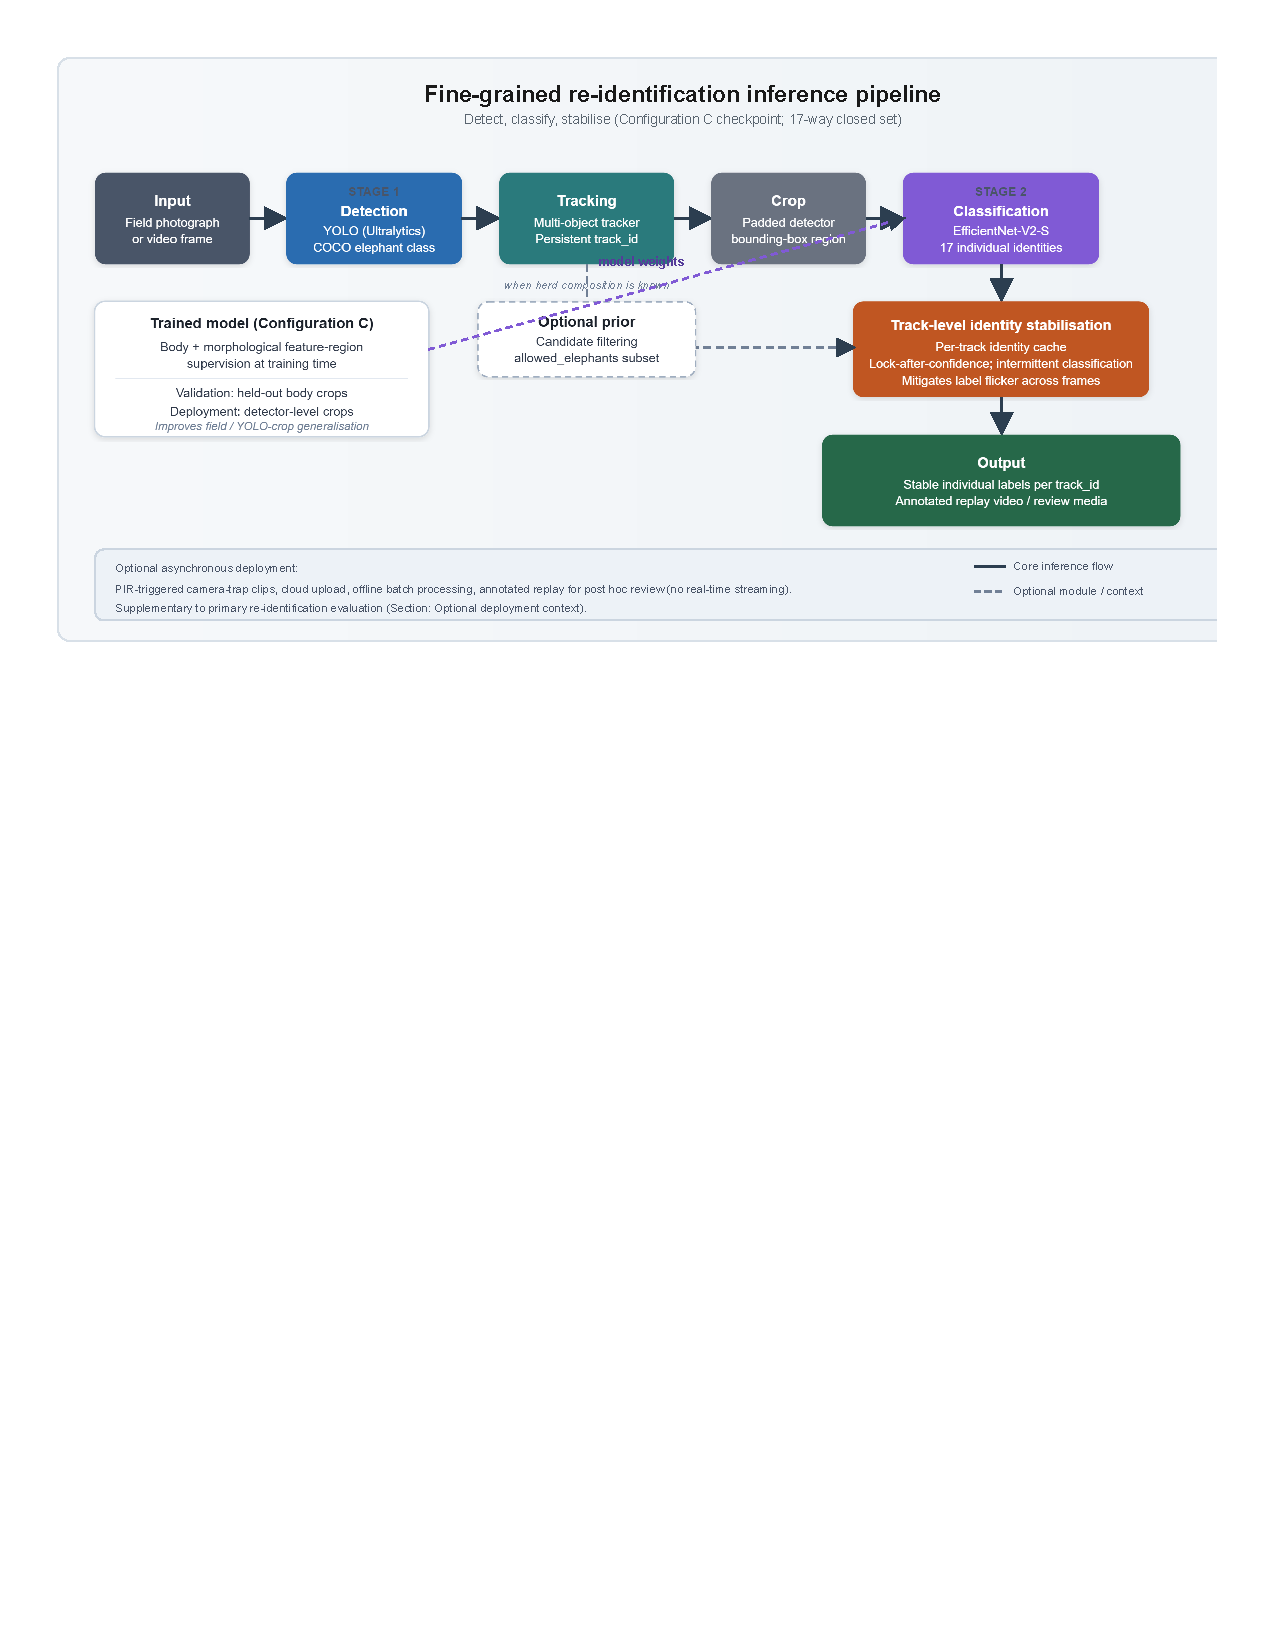
\includegraphics[width=0.92\linewidth]{figures/pipeline.pdf}
  \caption{Re-identification inference pipeline (supporting implementation): YOLO detection and multi-object tracking, EfficientNet-V2-S classification on padded detector crops, track-level identity stabilisation with optional candidate filtering, and annotated replay output. The Configuration~C checkpoint (body plus morphological feature-region supervision) is used at deployment. Vector source: \texttt{figures/pipeline.svg}; export PDF with \texttt{figures/export\_pipeline\_pdf.py}.}
  \label{fig:pipeline}
\end{figure}

\section{Discussion}
\label{sec:discussion}

This work centres on fine-grained re-identification methodology for Asian elephants. The three-configuration ablation highlights a methodological lesson: \textbf{reference-catalogue validation can be misleading}. Configurations~A and~B reached 99.85\% top-1 accuracy on held-out library body crops yet failed in the field---they had effectively learned catalogue appearance rather than stable identity-diagnostic morphology. Configuration~C addressed this library--field gap through morphological feature-region supervision (trunk, legs, ear folds, depigmentation patches), mirroring how human experts decompose an elephant into discriminative traits.

The body-plus-feature training strategy therefore improves \emph{generalisation}, not merely closed-set separability on curated portraits. Training on distributed morphological cues encourages invariance to framing, distance, and partial views---the dominant sources of domain shift between reference folders and YOLO crops at inference.

Track-level identity locking and candidate filtering address temporal inconsistency in video without requiring recurrent architectures. Restricting inference to expected individuals mirrors operational prior knowledge when daily herd composition is known.

The optional asynchronous camera-trap workflow (Section~\ref{sec:deployment}) shows that annotated replay can support \emph{post hoc} review after upload; it should not be interpreted as real-time monitoring. Classifier accuracy and upload latency are separate design considerations.

\subsection{Limitations}

\begin{enumerate}
  \item \textbf{Closed-set re-identification.} Unknown individuals may be misassigned; open-set rejection was not evaluated.
  \item \textbf{Validation domain shift.} High reference-library accuracy (Configuration~B: 99.85\%) did not predict field performance until the proposed body-plus-feature configuration; full quantitative evaluation on uploaded infrared clips remains to be completed.
  \item \textbf{Asynchronous workflow.} Reported camera-trap integration supports batch upload and post hoc review, not real-time identification.
  \item \textbf{Class imbalance.} Uneven reference counts may weaken reliability for under-sampled identities.
  \item \textbf{Cellular upload bias.} Where the optional upload workflow is used, monitoring effort may be constrained by 4G availability, independent of recognition performance.
  \item \textbf{Scalability.} Extending beyond ${\sim}$20 identities will increase annotation and confusion risk among similar animals.
\end{enumerate}

\section{Conclusion}
\label{sec:conclusion}

We presented a fine-grained re-identification approach for Asian elephants with morphological feature-region supervision. A three-configuration ablation showed that body-only training can reach 99.85\% reference-library validation accuracy yet fail in the field, whereas the proposed body-plus-feature configuration substantially improved in-situ and YOLO-crop re-identification. Morphological feature-region labelling supplies the supervisory mechanism enabling this generalisation gain.

\section*{Acknowledgements}

\textit{[Funding, facility staff, computing resources, and permissions.]}

\section*{Data and code availability}

Source code: \textit{[GitHub/Zenodo URL upon publication]}. Model weights and full training images: \textit{[available on request / restricted by facility policy]}.

\bibliographystyle{elsarticle-num}
\bibliography{references}

\end{document}
